
\newcommand{\sagadocument}{ExTENCI: SAGA Condor Integration}
\newcommand{\sagaversion}{1.0}
\newcommand{\sagabasename}{saga-programming-guide}
\newcommand{\sagaemail}{saga-users@cct.lsu.edu}

\documentclass{article}

\usepackage{ifpdf}

\ifpdf
  \usepackage[pdftex]{graphicx}
  \usepackage[pdftex]{hyperref}
  \DeclareGraphicsExtensions{.pdf, .png, .jpg}
  \graphicspath{{pics/}}
\else
  \usepackage{graphicx}
  \usepackage[hypertex]{hyperref}
  \DeclareGraphicsExtensions{.ps, .eps}
  \graphicspath{{pics/}}
\fi


\usepackage{srcltx}
\usepackage{fancyhdr}
\usepackage{wrapfig}
\usepackage{fancyvrb}
\usepackage{lscape}
\usepackage{color}
\usepackage{xspace}

\newcommand{\F}[1]{\textbf{#1}}
\newcommand{\B}[1]{\textbf{#1}}
\newcommand{\I}[1]{\textit{#1}}
\newcommand{\T}[1]{\texttt{#1}}
\newcommand{\U}[1]{\underline{#1}}

\newcommand{\BI}[1]{\B{\I{#1}}}
\newcommand{\BU}[1]{\B{\U{#1}}}

\newcommand{\X}[1]{\B{\U{FIXME: } #1}}

\newcommand{\LF}{Look\,\&\,Feel\xspace}

\newlength{\myflen} 

\newcommand{\XMark}[1][1]{%
  \setlength{\myflen}{1.2em}%
  \marginpar{\rule[-0.3em]{.5mm}{#1\myflen}}%
  \xspace%
}
\newcommand{\XRed}[1]{\textit{\textcolor{red}{\tiny #1}}}
\newcommand{\XGreen}[1]{\textbf{\textcolor{green}{#1}}}
\newcommand{\XBlue}[1]{\textit{\textcolor{blue}{#1}}}

% spelling fix
\newcommand{\XSpell}[2][1]{\XGreen{#2}\XMark[#1]}
\newcommand{\XSpelln}[1]{\XGreen{#1}}

% clarification fix
\newcommand{\XCorr}[2][1]{\XBlue{#2}\XMark[#1]}
\newcommand{\XCorrn}[1]{\XBlue{#1}}

% error fix
\newcommand{\XErr}[2][1]{\XGreen{#2}\XMark[#1]}
\newcommand{\XErrn}[1]{\XGreen{#1}}

% removed text
\newcommand{\XRem}[2][1]{\XRed{#2}\XMark[#1]}
\newcommand{\XRemn}[1]{\XRed{#1}}

% added text
\newcommand{\XAdd}[2][1]{\XCorr[#1]{#2}}
\newcommand{\XAddn}[1]{\XCorrn{#1}}

% comment
\newcommand{\XComm}[1]{\XRed{#1}}
\newcommand{\XCommn}[1]{\XComm{#1}}
\newcommand{\XCom}[1]{\XGreen{#1}}

% replace text
\newcommand{\XRep}[3][1]{\XRed{#2~}\XBlue{#3}\XMark[#1]}
\newcommand{\XRepn}[2]{\XRed{#1~}\XBlue{#2}}

\newcommand{\MUST}       {\T{MUST}\xspace}
\newcommand{\MUSTNOT}    {\T{MUST NOT}\xspace}
\newcommand{\REQUIRED}   {\T{REQUIRED}\xspace}
\newcommand{\SHALL}      {\T{SHALL}\xspace}
\newcommand{\SHALLNOT}   {\T{SHALL NOT}\xspace}
\newcommand{\SHOULD}     {\T{SHOULD}\xspace}
\newcommand{\SHOULDNOT}  {\T{SHOULD NOT}\xspace}
\newcommand{\RECOMMENDED}{\T{RECOMMENDED}\xspace}
\newcommand{\MAY}        {\T{MAY}\xspace}
\newcommand{\OPTIONAL}   {\T{OPTIONAL}\xspace}

\newcommand{\HINT}[1]{
\begin{center}
 \fbox{
  \parbox{.9\textwidth}{
   \B{HINT:}\\
    #1}}
\end{center}}

\newcommand{\sshift}{\hspace*{1em}}
\newcommand{\sunshift}{\hspace*{-1em}}
\newcommand{\shift}{\hspace*{3em}}
\newcommand{\unshift}{\hspace*{-3em}}
\newcommand{\down}{\vspace*{1em}}
\newcommand{\downn}{\vspace*{0.5em}}
\newcommand{\up}{\vspace*{-1em}}
\newcommand{\upp}{\vspace*{-0.5em}}

\setlength{\parskip}{1em}
\setlength{\parindent}{0em}
\setlength{\fboxsep}{1em}

\newcommand{\mywfig}[4]{
  \begin{wrapfigure}{#1}{#2\textwidth}
    \includegraphics[width=#2\textwidth]{#3}
    \caption{\label{fig:#3} #4}
    \vspace*{-1em}
  \end{wrapfigure}
}

\newcommand{\myfig}[2]{
  \begin{figure}[!ht]
    \begin{center}
      \includegraphics[width=0.95\textwidth]{#1}
      \caption{\label{fig:#1} #2}
    \end{center}
  \end{figure}
}


% \usepackage[titles]{tocloft}
%   \renewcommand{\cftbeforesecskip}{-0.0ex}
%   \renewcommand{\cftbeforesubsecskip}{-1ex}
%   \renewcommand{\cftbeforesubsubsecskip}{-1ex}
%   \renewcommand{\cftbeforetabskip}{-1ex}
%   \renewcommand{\cftbeforefigskip}{-1ex}

\setcounter{tocdepth}{2}

\pagestyle{fancy}
\pagenumbering{arabic}

\newcommand{\sagadate}{\today}

\newcommand{\sagaheader}{}
  \lhead{\sagadocument}
  \chead{\sagaheader}
  \rhead{\sagadate}
  \lfoot{\hrulefill\\\T{\sagaemail} \hfill \thepage}
  \cfoot{}
  \rfoot{}

\newcommand{\sagapart}[2]
{
  \part{#1}
  \label{part:#2}
  \renewcommand{\sagaheader}{#1}
  \input{\sagabasename_#2.tex}
}

\newcommand{\sagansec}[2]
{
  \section{#1}
  \label{sec:#2}
  \renewcommand{\sagaheader}{#1}
  \input{\sagabasename_#2.tex}
}

\newcommand{\sagannsec}[2]
{
  \section*{#1}
  \label{sec:#2}
  \renewcommand{\sagaheader}{#1}
  \input{\sagabasename_#2.tex}
}

\newcommand{\sagasec}[2]
{
  \section{#1}
  \label{sec:#2}
  \renewcommand{\sagaheader}{#1}
  \input{\sagabasename_#2.tex}
  \newpage
}

\newcommand{\sagassec}[2]
{
  \subsection{#1}
  \label{ssec:#2}
  \renewcommand{\sagaheader}{#1}
  \input{\sagabasename_#2.tex}
  \newpage
}

\newenvironment{shortlist}{
  \begin{itemize}
  \vspace*{-0.5em}
   \setlength{\itemsep}{-.1em}
}{
  \end{itemize}
}

\newenvironment{shortenum}{
  \begin{enumerate}
  \vspace*{-0.5em}
   \setlength{\itemsep}{-.1em}
}{
  \end{enumerate}
}

\DefineVerbatimEnvironment{mycode}{Verbatim}
{
  label=Code Example,
  fontsize=\small,
  frame=single,
% framerule=1pt,
  framesep=1em,
% numbers=left,
  gobble=2
}


\DefineVerbatimEnvironment{myio}{Verbatim}
{
  fontsize=\small,
  frame=lines,
% framerule=1pt,
  framesep=1em
}


\DefineVerbatimEnvironment{mysmallspec}{Verbatim}
{
  fontsize=\small,
  frame=lines,
% framerule=1pt,
  framesep=1em
}

\DefineVerbatimEnvironment{myspec}{Verbatim}
{
  fontsize=\normalsize,
  frame=lines,
% framerule=1pt,
  framesep=1em
}


\newcommand{\sagabib}[1]{
  \renewcommand{\sagaheader}{References}
  \addcontentsline{toc}{section}{References}
  \label{sec:References}
  \bibliographystyle{abbrv}
  \bibliography{#1}
}



\newcommand{\name}{\F{SAGA}\xspace}
\DefineShortVerb{\|}

\begin{document}

 \thispagestyle{empty}

 \sagadocument\hfill  Ole Weidner, CCT/LSU\\
  Version: \sagaversion \hfill {\sagadate}


  \hrulefill\\[2em]

  \B{\large ExTENCI: SAGA Condor Integration}\\[4em]



  %\U{Abstract}

   The aim of this document is to describe the use-cases and requirements 
   for a possible integration of SAGA and Condor. Based on these requirements, 
   an implementation concept for a Condor plug-in for SAGA (\textit{Adatpor}) is 
   derived and described in detail. 
   With this proposed \textit{Condor Adaptor}, it will be possible to use Condor,
   Condor-G as
   well as Condor glide-in programmatically through the standardized SAGA C++ and 
   Python interfaces.
   
   This project is part of the the Extending Science Through Enhanced National 
   Cyberinfrastructure (ExTENCI) project, which is a joint Open Science Grid (OSG)
   and TeraGrid project, funded by the National Science Foundation Office of 
   Cyberinfrastructure (NSF OCI).
   \\[2em]


  \U{Status of This Document}

  This document is still work in progress.\\
  
    \U{Copyright Notice}

  Copyright \copyright~T.B.D (2011).  All Rights
  Reserved.\\

  \newpage

  \tableofcontents

  \newpage

%-----------------------------------------------------------------
% Intro, structure, disclaimer, ...
%-----------------------------------------------------------------
                                        
\section {SAGA}

\begin{figure}
  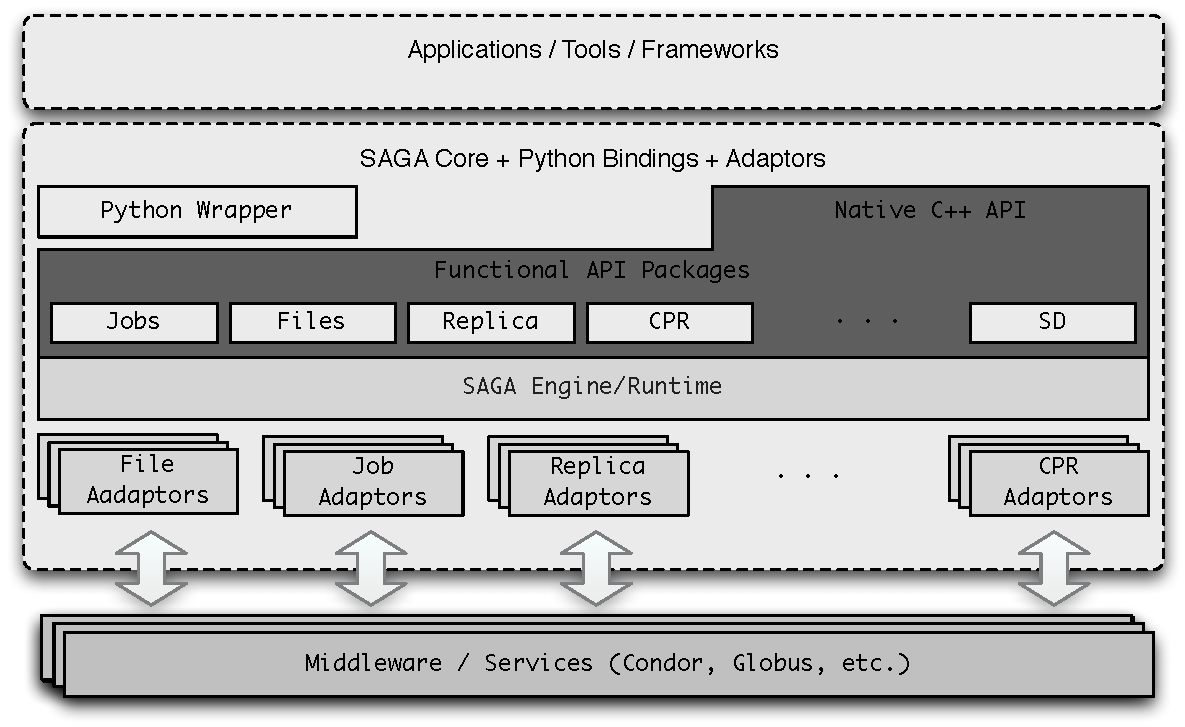
\includegraphics[width=1.0\textwidth]{./figures/figure_02}
  \caption{\footnotesize Layered schematic of the different
    components of SAGA.  Middleware specific adaptors make
    applications developed using SAGA portable.  Schematic showing the
    different ways in which SAGA can be used to develop distributed
    applications. (i) Using native SAGA calls to implement distributed
    functionality; (ii) Through the use of frameworks which provide
    either application-level usage modes, patterns and thus shielding
    the application from directly interfacing with the
    infrastructure.}
%\vspace{-1em}
 \label{sagalayer}
\end{figure}
	
	
\subsection{API Specification}	
A set of application groups expressed the desire for a 
simple programmatic interface that would be widely-adopted and widely-available,
which led to the need and role for the SAGA API. 
The goal of such an interface is to provide a ``distributed computing 
counterpart to MPI'' (in impact if not in details), 
and to supply developers with
a simple, uniform, and standard programmatic interface with which to
develop applications.  Thanks to the efforts of many contributors, an initial 
specification of such an interface was released in 2008: the Simple API for Grid
Applications (OGF-GFD-90). The scope and requirements of
the SAGA API have been formally defined by OGF's SAGA Research Group
(SAGA-RG). The SAGA-RG collected use cases from a broad user
community and published them as OGF-GFD.70. The
requirements and design for the SAGA API were directly derived from
these use cases; this process has been documented and published in
OGF-GFD.71. The end result of this process is the 1.0
version of the SAGA core specification (OGF-GFD.90),
which defines language-independent syntax and semantics for the SAGA
core API (error handling, session and context management, permissions,
monitoring, attribute and task model) and functional packages (jobs,
name-spaces, files, replicas, streams, RPC). Several API extension,
such as CPR (OGF-GWD-R.96), Adverts
(GFD-R-P.XX~), and Messaging (GWD-R.94) are currently under development and
follow a similar, well-defined community-driven standardization and
approval process. SAGA is now an Open Grid Forum (OGF)
proposed recommendation on the path to becoming a standard.  The
standardization is important because
it makes it more likely that infrastructures will support
SAGA, which may make it widely available for users of
most national CI projects.
	
\subsection{C++/Python Implementation}
The SAGA implementation referred to in this 
document is an implementation of the SAGA API Specification written in C++ 
and Python. SAGA is open source software, released under the Boost Software
License. It can be divided into three major components (as depicted in Fig. \ref{sagalayer}): the \I{Core
Components} which provide the API functionality, the \I{Adaptors}
which translate API calls into native middleware calls, the Python API
\I{Language Bindings} and a set of \I{Command Line Tools}. The SAGA
\I{Core Components} are a collection of dynamic libraries and header
files that represent the functional API packages (see section 2.1)
along with a lightweight, highly-configurable \I{Engine Component}
that manages call dispatching and the dynamic runtime loading of the
\I{Middleware Adaptors}.

SAGA is being actively developed by our group at Louisiana State University
with many contributions from external groups and collaborators. More information
about SAGA can be found on the website: http://saga.cct.lsu.edu.


	
	
\section {Condor}
	
\subsection{Condor-G}
	
\subsection{Condor Glide-in}

\section {Integration}

\subsection{Use-Cases}
These are the use-cases that have been identified within the ExTENCI project. The
final outcome of this integration project will be tested against these use-cases
to make sure that the implementation is feature-complete.

\begin{itemize}
\item \textbf{U.01:} A user submits, monitors and controls Condor jobs through
the SAGA Job API.

\item \textbf{U.02:} A user can select Condor-G ("Globus via Condor") resources
as well as regular Condor pools for job execution through the SAGA Job API.

\item \textbf{U.03:}

\end{itemize}

\subsection{Requirements}

In addition to the use-cases, we define a set of requirements that the 
implementation has to fulfill:

\begin{itemize}
\item \textbf{R.01:} E.g. stuff like types of system where this has to work, etc.
\end{itemize}

\subsection{Adaptor Architecture}

\begin{figure}
  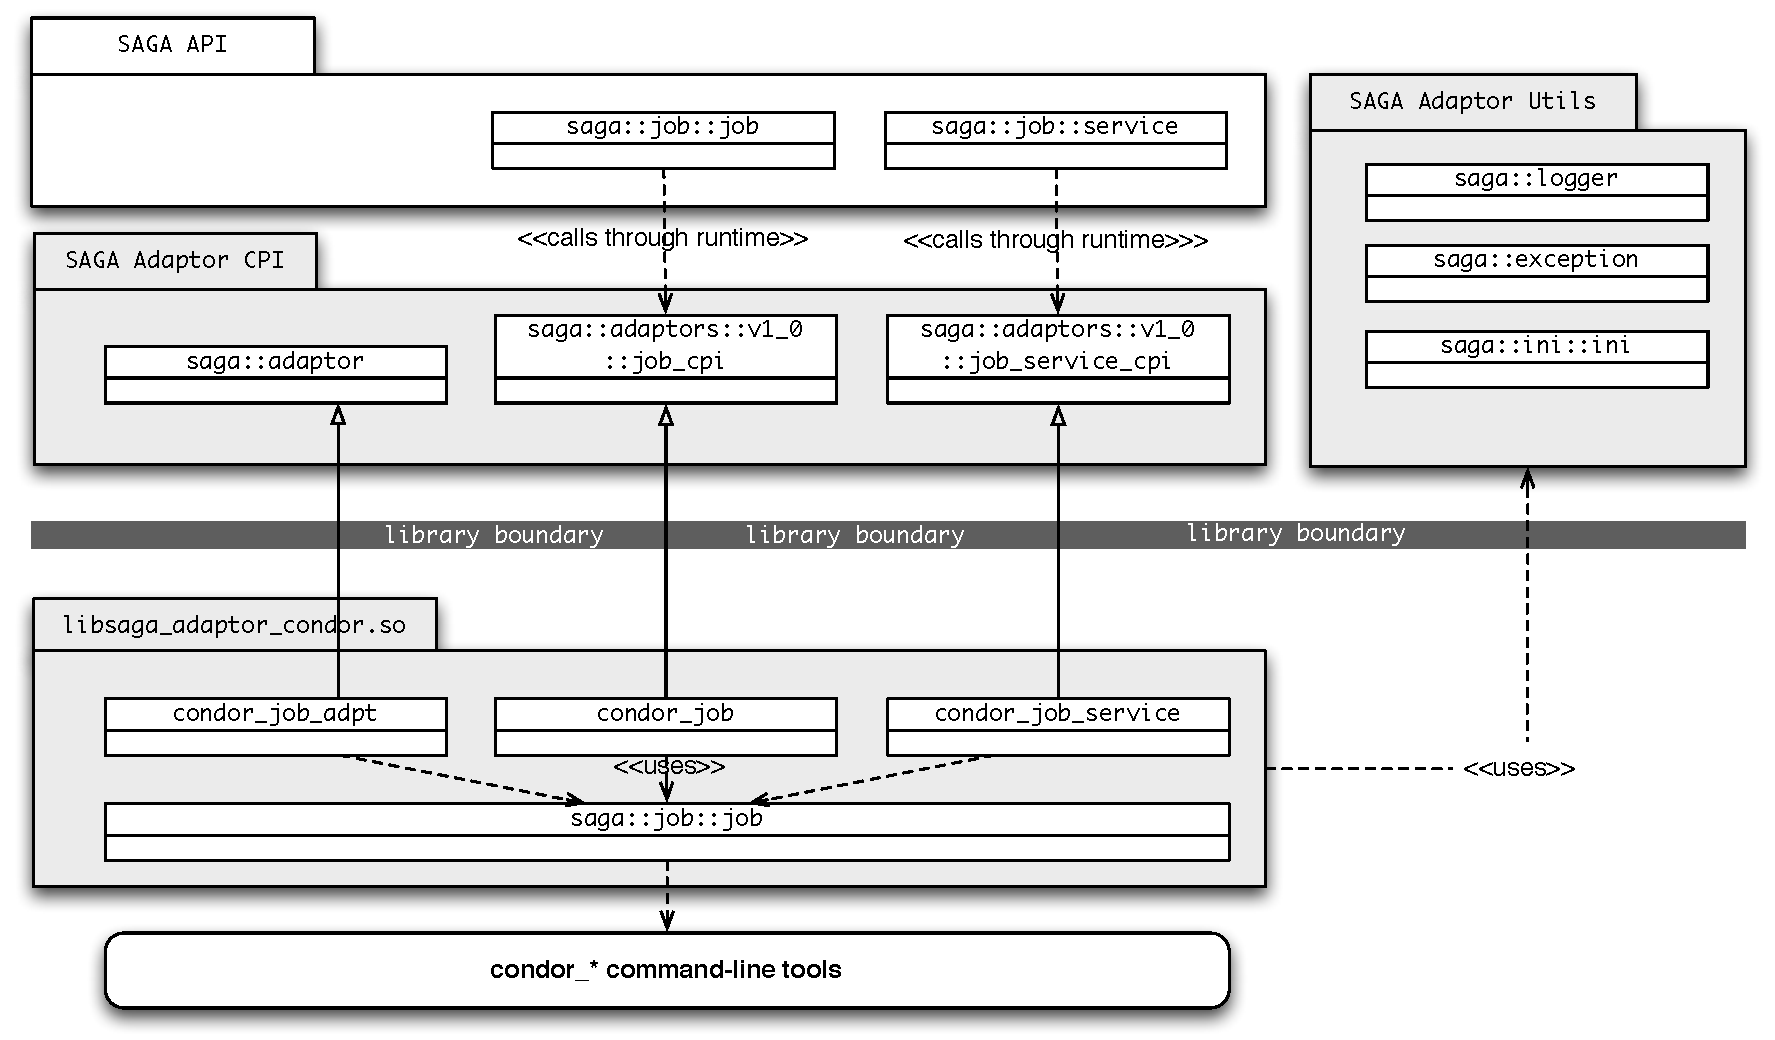
\includegraphics[width=1.0\textwidth]{./figures/condor_adaptor_arch}
  \caption{\footnotesize The SAGA Condor adaptor architecture. The adaptor interfaces
  with SAGA's well defined Capability Provider Interface (CPI), or \textit{Adaptor API}.
  This ensures that the adaptor fully integrates with SAGA's intelligent adaptor selection
  mechanism, logging and error handling facilities. To ensure maximum versatility across
  platforms, the Condor adaptors uses the boost::process API to call the Condor command 
  line tools. }
  
%\vspace{-1em}
 \label{sagalayer}
\end{figure}

\end{document}


